% 要由本.tex文件编译得到对应的.pdf文档,请使用xetex连续编译两次
\documentclass[nogbt]{my_cumcmthesis}
\usepackage{booktabs} %用于绘制三线表
\usepackage{graphicx} %用于插入图片
\usepackage{subcaption} %用于插入子图
\usepackage{metalogo} %用于表现XeLaTeX的LOGO
\usepackage{zhlipsum} %用于检测排版
\usepackage{amsmath,amssymb} %数学相关

\title{基于ctexart的数学建模国赛论文模板} %论文标题
\author{Zhihao Ye} %作者(可填可不填)
\date{2023/08/12} %日期(可填可不填)

\begin{document}
\maketitle %生成封面页
\begin{abstract}
    \colorbox{gray!15}{\lstinline!my\_cumthesis.cls.tex!}是笔者为\textbf{全国大学生数学建模竞赛}而编写的\LaTeX{}模板。现在你阅读的是该模板的样例文档。
    
    考虑到移植性问题,本模板设计得较为轻量,所以使用者需要有一定的\LaTeX{}使用经验。此参考文档由\colorbox{gray!15}{\lstinline!基于ctexart的数学建模国赛论文模板.tex!}文件经过\XeLaTeX{}编译得到。下面是本模板主要做出的简化工作。

    \textbf{预先全局导入了部分常用的宏包},包括但不限于\AmS{}部分数学宏包,支持中文的\CTeX{}宏集等,使导言区更加简洁。

    \textbf{预设置或重定义了各种排版细节},包括但不限于摘要环境、各级标题、附录代码块等,使论文格式达到国赛的要求。

    \textbf{新定义了各种命令和环境},包括但不限于关键词命令、定理类环境等,增加论文书写的效率。

    \keywords{\LaTeX{} \quad \CTeX \quad 数学建模}
\end{abstract}

\section{问题重述}

\begin{description}
    \item[问题一] 这里是对问题一的精简重述。
    \item[问题二] 这里是对问题二的精简重述。
    \item[问题三] 这里是对问题三的精简重述。
    \item[问题四] 这里是对问题四的精简重述。
\end{description}

\section{问题分析}
\subsection{问题一}
    \zhlipsum[1] %用废话测试排版
\subsection{问题二}
    \zhlipsum[2] %用废话测试排版
\subsection{问题三}
    \zhlipsum[3-4] %用废话测试排版
\subsection{问题四}
    \zhlipsum[5] %用废话测试排版

\section{模型假设}
\begin{enumerate}
    \item 这里是假设一。
    \item 这里是假设二。
\end{enumerate}

\section{符号说明}
\begin{center}\begin{tabular}{cc}
    \toprule
    符号 & 含义 \\
    \midrule
    $\mathbb{R}$ & 实数 \\
    $f$ & 函数$f$ \\
    $F$ & $f$的原函数$F$ \\
    \bottomrule
\end{tabular}\end{center}

\section{模型的建立与求解}
\subsection{问题一的模型建立与求解}
\subsubsection{问题一模型的建立}
    \zhlipsum[6-7] %用废话测试排版
    \begin{figure}[hbp]
        \centering
        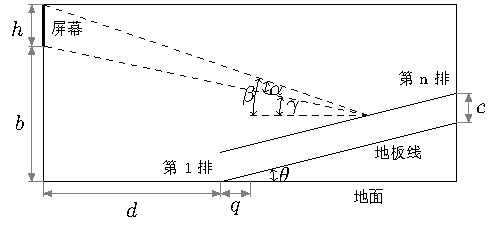
\includegraphics{source/影院纵向剖面示意图.pdf}
        \caption{实例图片一\upcite{jiangqiyuan}}
        \label{fig:eg1}
    \end{figure}
    \zhlipsum[8] %用废话测试排版

\subsubsection{问题一模型的求解}
    \zhlipsum[9] %用废话测试排版

\subsection{问题二的模型建立与求解}
\subsubsection{数据预处理}
    经过处理后样例数据如下表所示\upcite{sishoukui}。
\begin{table}[htbp]
    \centering
    \begin{tabular}{*{4}{|c|c|}}
        \hline
        经度	 & 维度		 & 经度		& 维度		  & 维度	 & 经度		  & 维度	   & 维度 	 \\ \hline
        53.7121	& 15.3046	& 51.1758  & 0.0322	 	& 46.3253  & 28.2753	& 30.3313   & 6.9348  \\ \hline
        56.5432 & 21.4188	& 10.8198  & 16.2529 	& 22.7891  & 23.1045	& 10.1584   & 12.4819 \\ \hline
        20.1050 & 15.4562	& 1.9451   & 0.2057	 	& 26.4951  & 22.1221	& 31.4847   & 8.9640  \\ \hline
        26.2418 & 18.1760	& 44.0356  & 13.5401 	& 28.9836  & 25.9879	& 38.4722   & 20.1731 \\ \hline
        28.2694 & 29.0011	& 32.1910  &  5.8699	& 36.4863  & 29.7284	& 0.9718    & 28.1477 \\ \hline
        8.9586  & 24.6635	& 16.5618  & 23.6143	& 10.5597  & 15.1178	& 50.2111   & 10.2944 \\ \hline
        8.1519  & 9.5325	& 22.1075  & 18.5569	& 0.1215   & 18.8726	& 48.2077   & 16.8889 \\ \hline
        31.9499 & 17.6309	& 0.7732   & 0.4656		& 47.4134  & 23.7783	& 41.8671   & 3.5667  \\ \hline
        43.5474 & 3.9061	& 53.3524  & 26.7256	& 30.8165  & 13.4595	& 27.7133   & 5.0706  \\ \hline
        23.9222 & 7.6306	& 51.9612  & 22.8511	& 12.7938  & 15.7307	& 4.9568    & 8.3669  \\ \hline
        21.5051 & 24.0909	& 15.2548  & 27.2111	& 6.2070   & 5.1442		& 49.2430   & 16.7044 \\ \hline
        17.1168 & 20.0354	& 34.1688  & 22.7571	& 9.4402   & 3.9200		& 11.5812   & 14.5677 \\ \hline
        52.1181 & 0.4088	& 9.5559   & 11.4219	& 24.4509  & 6.5634		& 26.7213   & 28.5667 \\ \hline
        37.5848 & 16.8474	& 35.6619  & 9.9333		& 24.4654  & 3.1644		& 0.7775    & 6.9576  \\ \hline
        14.4703 & 13.6368	& 19.8660  & 15.1224	& 3.1616   & 4.2428		& 18.5245   & 14.3598 \\ \hline
        58.6849 & 27.1485	& 39.5168  & 16.9371	& 56.5089  & 13.7090	& 52.5211   & 15.7957 \\ \hline
        38.4300 & 8.4648	& 51.8181  & 23.0159	& 8.9983   & 23.6440	& 50.1156   & 23.7816 \\ \hline
        13.7909 & 1.9510	& 34.0574  & 23.3960	& 23.0624  & 8.4319		& 19.9857   & 5.7902  \\ \hline
        40.8801 & 14.2978	& 58.8289  & 14.5229	& 18.6635  & 6.7436		& 52.8423   & 27.2880 \\ \hline
        39.9494 & 29.5114	& 47.5099  & 24.0664	& 10.1121  & 27.2662	& 28.7812   & 27.6659 \\ \hline
        8.0831  & 27.6705	& 9.1556   & 14.1304	& 53.7989  & 0.2199		& 33.6490   & 0.3980  \\ \hline
        1.3496  & 16.8359	& 49.9816  & 6.0828		& 19.3635  & 17.6622	& 36.9545   & 23.0265 \\ \hline
        15.7320 & 19.5697	& 11.5118  & 17.3884	& 44.0398  & 16.2635	& 39.7139   & 28.4203 \\ \hline
        6.9909  & 23.1804	& 38.3392  & 19.9950	& 24.6543  & 19.6057	& 36.9980   & 24.3992 \\ \hline
        4.1591  & 3.1853	& 40.1400  & 20.3030	& 23.9876  & 9.4030		& 41.1084   & 27.7149 \\ \hline
    \end{tabular}
    \caption{实例数据表}
    \label{tab:eg}
\end{table}

\subsubsection{问题二模型的建立}
    \zhlipsum[10] %用废话测试排版

\subsubsection{问题二模型的求解}
    按照上述算法,经过计算机程序计算可以得到如下结果。
    \begin{figure}[htbp]
        \centering
        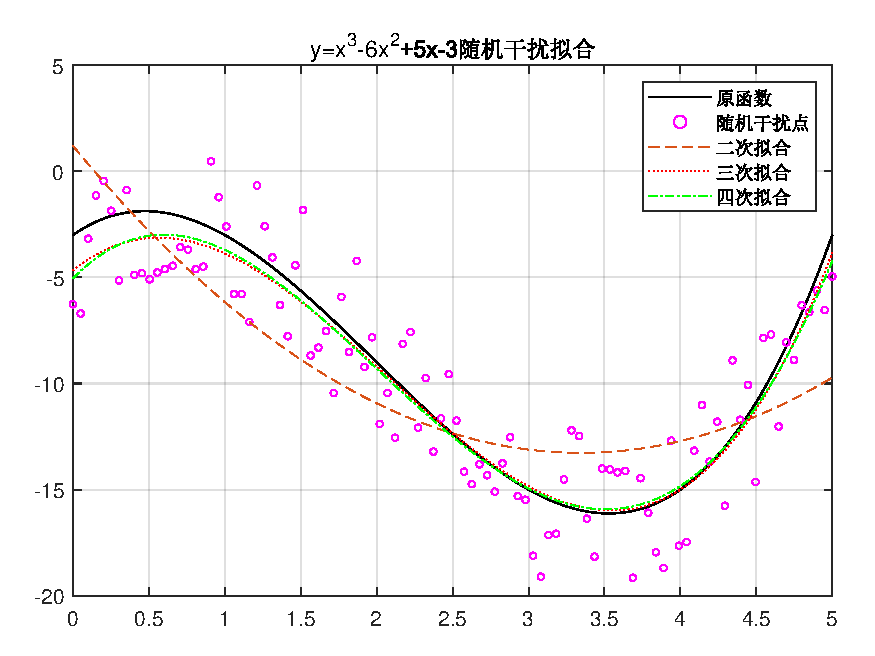
\includegraphics[scale=0.8]{source/FunctionFitting.pdf}
        \caption{实例图片二}
        \label{fig:eg2}
    \end{figure}

\subsection{问题三的模型建立与求解}
\subsubsection{问题三模型的建立}
   如下是多幅图像的并排展示。
    \begin{figure}[htbp] %测试多图并列
        \centering
        \begin{minipage}[c]{0.48\textwidth}
            \centering
            
\includegraphics[scale=0.45]{source/朋友.jpg} %图像高度要预先统一
            \subcaption{朋友}
            \label{fig:friends}
        \end{minipage}
        \begin{minipage}[c]{0.48\textwidth}
            \centering
            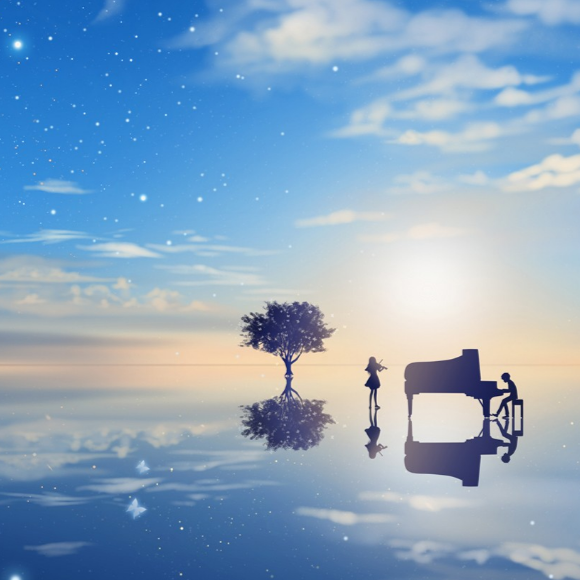
\includegraphics[scale=0.45]{source/合奏.png}
            \subcaption{合奏}
            \label{fig:duet}
        \end{minipage}
        \caption{多图并排实例}
        \label{fig:eg3}
    \end{figure}
\subsubsection{问题三模型的求解}
    这里是模型解答结果。
\subsection{问题四}
    我们先不加证明地给出如下的众所周知公理。
    \begin{lemma}[众所周知公理]
        众所周知,
        \begin{equation}
            1 + 1 = 2.
            \label{eq:1}
        \end{equation}
        \label{lma:wellknown}
    \end{lemma}
    对问题四的解答需要如下的定理\upcite{zhuoliqi}。
    \begin{theorem}[Newton-Leibniz 公式]
        如果$f:\ [a,b] \rightarrow \mathbb{R}$是只有有限个间断点的有限函数,则$f\in R[a,b]$,并且
    \begin{equation}
        \int_{a}^{b}f(x)\mathrm{d}x = F(b) - F(a),
        \label{eq:2}
    \end{equation}
    其中$F:\ [a,b] \rightarrow \mathbb{R}$是函数$f$在闭区间$[a,b]$上的任何一个原函数。
    \label{thm:NL}
    \end{theorem}
    \begin{proof}
        观察式\eqref{eq:1},我们注意到,式\eqref{eq:2}是十分重要且显而易见的。
    \end{proof}
    通过上面的分析,我们发现问题四在上面的假设情况下是无解的。

\section{模型评价}
    为保护文学、艺术和科学作品作者的著作权,以及与著作权有关的权益,鼓励有益于社会主义精神文明、物质文明建设的作品的创作和传播,促进社会主义文化和科学事业的发展与繁荣,根据宪法制定《中华人民共和国著作权法》\upcite{zhuzuoquanfa}。
    
    显然该模型还有改进的空间。
\newpage

\begin{thebibliography}{9}
    \bibitem[1]{liuhaiyang}
    刘海洋.
    \newblock \LaTeX {}入门\allowbreak[M].
    \newblock 北京: 电子工业出版社, 2013.

    \bibitem[2]{jiangqiyuan}
    姜启源, 谢金星, 叶俊.
    \newblock 数学模型(第五版)\allowbreak[M].
    \newblock 北京: 高等教育出版社, 2018.

    \bibitem[3]{sishoukui}
    司守奎,孙玺菁.
    \newblock 数学建模算法与应用(第三版)\allowbreak[M].
    \newblock 北京: 国防工业出版社, 2021.

    \bibitem[4]{zhuoliqi}
    (俄罗斯)B.A.卓里奇.
    \newblock 数学分析:第七版.第一卷\allowbreak[M].
    \newblock 李植. 北京: 高等教育出版社, 2019.

    \bibitem[5]{zhuzuoquanfa}
    中国人大网.
    \newblock 中华人民共和国著作权法\allowbreak[EB/OL].
    \newblock (2020-11-11)[2023-08-05].
    \newblock \url{http://www.gov.cn/guoqing/2021-10/29/content_5647633.htm}
\end{thebibliography}
\newpage

\begin{appendix}
\section{支撑材料}
    文件列表如下。
\begin{lstlisting}
    functionFitting.m
    FunctionFitting.pdf
    全国大学生数学建模竞赛论文格式规范.doc
    合奏.png
    朋友.jpg
    影院纵向剖面示意图.pdf
\end{lstlisting}

\section{相关代码}
\begin{lstlisting}[language=matlab]
    % functionFitting.m
    % 基于y = x^3 - 6x^2 + 5x - 3产生含有随机干扰的数据
    close all; clear; clc;
    xi = linspace(0,5);
    y = xi.^3 -  6.*xi.^2 + 5.*xi - 3;
    yi = y + 8 .* rand(1,100) - 4; %干扰均匀分布在[-4,4]
    plot(xi,y,'k-','LineWidth',0.75);
    hold on; grid on;
    scatter(xi,yi,10,'m');
    
    % 拟合随机数据2次
    f2 = polyfit(xi,yi,2);
    fy = polyval(f2,xi);
    plot(xi,fy,'--','Color',[0.8500 0.3250 0.0980]);
    
    % 拟合随机数据3次
    f3 = polyfit(xi,yi,3);
    fy = polyval(f3,xi);
    plot(xi,fy,'r:');
    
    % 拟合随机数据4次
    f4 = polyfit(xi,yi,4);
    fy = polyval(f4,xi);
    plot(xi,fy,'g-.');
    
    title('y=x^3-6x^2+5x-3随机干扰拟合');
    legend('原函数','随机干扰点','二次拟合','三次拟合','四次拟合');
\end{lstlisting}
\end{appendix}

\end{document}